\begin{tikzpicture}
    \draw[fill=orange!40] (0,0) ellipse (3 and 1.8);
    \draw[fill=cyan!40] (-.9,-.3) ellipse (1.5 and 1);
    \node at (-.9,-.3) {Ricorsivi};
    \node at (0.05,1) {Ricorsivamente numerabili};
    \node at (1.7,-.3) {$\underset{\text{\textbullet}}{A}$};
    \node at (3.7,.2) {$\underset{\text{\textbullet}}{A^c}$};
    \draw (4.8,-1.9) -- (4.8,1.9);
\end{tikzpicture}